\documentclass[twoside]{book}

% Packages required by doxygen
\usepackage{fixltx2e}
\usepackage{calc}
\usepackage{doxygen}
\usepackage[export]{adjustbox} % also loads graphicx
\usepackage{graphicx}
\usepackage[utf8]{inputenc}
\usepackage{makeidx}
\usepackage{multicol}
\usepackage{multirow}
\PassOptionsToPackage{warn}{textcomp}
\usepackage{textcomp}
\usepackage[nointegrals]{wasysym}
\usepackage[table]{xcolor}

% Font selection
\usepackage[T1]{fontenc}
\usepackage[scaled=.90]{helvet}
\usepackage{courier}
\usepackage{amssymb}
\usepackage{sectsty}
\renewcommand{\familydefault}{\sfdefault}
\allsectionsfont{%
  \fontseries{bc}\selectfont%
  \color{darkgray}%
}
\renewcommand{\DoxyLabelFont}{%
  \fontseries{bc}\selectfont%
  \color{darkgray}%
}
\newcommand{\+}{\discretionary{\mbox{\scriptsize$\hookleftarrow$}}{}{}}

% Page & text layout
\usepackage{geometry}
\geometry{%
  a4paper,%
  top=2.5cm,%
  bottom=2.5cm,%
  left=2.5cm,%
  right=2.5cm%
}
\tolerance=750
\hfuzz=15pt
\hbadness=750
\setlength{\emergencystretch}{15pt}
\setlength{\parindent}{0cm}
\setlength{\parskip}{3ex plus 2ex minus 2ex}
\makeatletter
\renewcommand{\paragraph}{%
  \@startsection{paragraph}{4}{0ex}{-1.0ex}{1.0ex}{%
    \normalfont\normalsize\bfseries\SS@parafont%
  }%
}
\renewcommand{\subparagraph}{%
  \@startsection{subparagraph}{5}{0ex}{-1.0ex}{1.0ex}{%
    \normalfont\normalsize\bfseries\SS@subparafont%
  }%
}
\makeatother

% Headers & footers
\usepackage{fancyhdr}
\pagestyle{fancyplain}
\fancyhead[LE]{\fancyplain{}{\bfseries\thepage}}
\fancyhead[CE]{\fancyplain{}{}}
\fancyhead[RE]{\fancyplain{}{\bfseries\leftmark}}
\fancyhead[LO]{\fancyplain{}{\bfseries\rightmark}}
\fancyhead[CO]{\fancyplain{}{}}
\fancyhead[RO]{\fancyplain{}{\bfseries\thepage}}
\fancyfoot[LE]{\fancyplain{}{}}
\fancyfoot[CE]{\fancyplain{}{}}
\fancyfoot[RE]{\fancyplain{}{\bfseries\scriptsize Generated by Doxygen }}
\fancyfoot[LO]{\fancyplain{}{\bfseries\scriptsize Generated by Doxygen }}
\fancyfoot[CO]{\fancyplain{}{}}
\fancyfoot[RO]{\fancyplain{}{}}
\renewcommand{\footrulewidth}{0.4pt}
\renewcommand{\chaptermark}[1]{%
  \markboth{#1}{}%
}
\renewcommand{\sectionmark}[1]{%
  \markright{\thesection\ #1}%
}

% Indices & bibliography
\usepackage{natbib}
\usepackage[titles]{tocloft}
\setcounter{tocdepth}{3}
\setcounter{secnumdepth}{5}
\makeindex

% Hyperlinks (required, but should be loaded last)
\usepackage{ifpdf}
\ifpdf
  \usepackage[pdftex,pagebackref=true]{hyperref}
\else
  \usepackage[ps2pdf,pagebackref=true]{hyperref}
\fi
\hypersetup{%
  colorlinks=true,%
  linkcolor=blue,%
  citecolor=blue,%
  unicode%
}

% Custom commands
\newcommand{\clearemptydoublepage}{%
  \newpage{\pagestyle{empty}\cleardoublepage}%
}

\usepackage{caption}
\captionsetup{labelsep=space,justification=centering,font={bf},singlelinecheck=off,skip=4pt,position=top}

%===== C O N T E N T S =====

\begin{document}

% Titlepage & ToC
\hypersetup{pageanchor=false,
             bookmarksnumbered=true,
             pdfencoding=unicode
            }
\pagenumbering{alph}
\begin{titlepage}
\vspace*{7cm}
\begin{center}%
{\Large Vid\+Chaser \\[1ex]\large 2.\+4.\+20170727 }\\
\vspace*{1cm}
{\large Generated by Doxygen 1.8.13}\\
\end{center}
\end{titlepage}
\clearemptydoublepage
\pagenumbering{roman}
\tableofcontents
\clearemptydoublepage
\pagenumbering{arabic}
\hypersetup{pageanchor=true}

%--- Begin generated contents ---
\chapter{Namespace Index}
\section{Namespace List}
Here is a list of all namespaces with brief descriptions\+:\begin{DoxyCompactList}
\item\contentsline{section}{\hyperlink{namespace_vid_chaser}{Vid\+Chaser} }{\pageref{namespace_vid_chaser}}{}
\end{DoxyCompactList}

\chapter{Class Index}
\section{Class List}
Here are the classes, structs, unions and interfaces with brief descriptions\+:\begin{DoxyCompactList}
\item\contentsline{section}{\hyperlink{class_matrix_util}{Matrix\+Util} }{\pageref{class_matrix_util}}{}
\item\contentsline{section}{\hyperlink{class_shader_util}{Shader\+Util} }{\pageref{class_shader_util}}{}
\end{DoxyCompactList}

\chapter{File Index}
\section{File List}
Here is a list of all files with brief descriptions\+:\begin{DoxyCompactList}
\item\contentsline{section}{C\+:/\+Workspace/\+Vid\+Chaser/\+Platform/\+Vid\+Chaser\+Android/\+Vid\+Chaser/src/main/java/com/maxst/vidchaser/\hyperlink{_camera1_controller_8java}{Camera1\+Controller.\+java} }{\pageref{_camera1_controller_8java}}{}
\item\contentsline{section}{C\+:/\+Workspace/\+Vid\+Chaser/\+Platform/\+Vid\+Chaser\+Android/\+Vid\+Chaser/src/main/java/com/maxst/vidchaser/\hyperlink{_camera2_controller_8java}{Camera2\+Controller.\+java} }{\pageref{_camera2_controller_8java}}{}
\item\contentsline{section}{C\+:/\+Workspace/\+Vid\+Chaser/\+Platform/\+Vid\+Chaser\+Android/\+Vid\+Chaser/src/main/java/com/maxst/vidchaser/\hyperlink{_camera_controller_8java}{Camera\+Controller.\+java} }{\pageref{_camera_controller_8java}}{}
\item\contentsline{section}{C\+:/\+Workspace/\+Vid\+Chaser/\+Platform/\+Vid\+Chaser\+Android/\+Vid\+Chaser/src/main/java/com/maxst/vidchaser/\hyperlink{_camera_size_8java}{Camera\+Size.\+java} }{\pageref{_camera_size_8java}}{}
\item\contentsline{section}{C\+:/\+Workspace/\+Vid\+Chaser/\+Platform/\+Vid\+Chaser\+Android/\+Vid\+Chaser/src/main/java/com/maxst/vidchaser/\hyperlink{_camera_surface_view_8java}{Camera\+Surface\+View.\+java} }{\pageref{_camera_surface_view_8java}}{}
\item\contentsline{section}{C\+:/\+Workspace/\+Vid\+Chaser/\+Platform/\+Vid\+Chaser\+Android/\+Vid\+Chaser/src/main/java/com/maxst/vidchaser/\hyperlink{_on_new_camera_frame_callback_8java}{On\+New\+Camera\+Frame\+Callback.\+java} }{\pageref{_on_new_camera_frame_callback_8java}}{}
\item\contentsline{section}{C\+:/\+Workspace/\+Vid\+Chaser/\+Platform/\+Vid\+Chaser\+Android/\+Vid\+Chaser/src/main/java/com/maxst/vidchaser/\hyperlink{_projection_matrix_8java}{Projection\+Matrix.\+java} }{\pageref{_projection_matrix_8java}}{}
\item\contentsline{section}{C\+:/\+Workspace/\+Vid\+Chaser/\+Platform/\+Vid\+Chaser\+Android/\+Vid\+Chaser/src/main/java/com/maxst/vidchaser/\hyperlink{_surface_manager_8java}{Surface\+Manager.\+java} }{\pageref{_surface_manager_8java}}{}
\item\contentsline{section}{C\+:/\+Workspace/\+Vid\+Chaser/\+Platform/\+Vid\+Chaser\+Android/\+Vid\+Chaser/src/main/java/com/maxst/vidchaser/\hyperlink{_vid_chaser_a_p_i_8java}{Vid\+Chaser\+A\+P\+I.\+java} }{\pageref{_vid_chaser_a_p_i_8java}}{}
\item\contentsline{section}{C\+:/\+Workspace/\+Vid\+Chaser/\+Platform/\+Vid\+Chaser\+Android/\+Vid\+Chaser/src/main/java/com/maxst/vidchaser/\hyperlink{_vid_chaser_j_n_i_8java}{Vid\+Chaser\+J\+N\+I.\+java} }{\pageref{_vid_chaser_j_n_i_8java}}{}
\end{DoxyCompactList}

\chapter{Namespace Documentation}
\hypertarget{namespacecom}{}\section{Package com}
\label{namespacecom}\index{com@{com}}
\subsection*{Packages}
\begin{DoxyCompactItemize}
\item 
package \hyperlink{namespacecom_1_1maxst}{maxst}
\end{DoxyCompactItemize}

\hypertarget{namespacecom_1_1maxst}{}\section{Package com.\+maxst}
\label{namespacecom_1_1maxst}\index{com.\+maxst@{com.\+maxst}}
\subsection*{Packages}
\begin{DoxyCompactItemize}
\item 
package \hyperlink{namespacecom_1_1maxst_1_1vidchaser}{vidchaser}
\end{DoxyCompactItemize}

\hypertarget{namespacecom_1_1maxst_1_1vidchaser}{}\section{Package com.\+maxst.\+vidchaser}
\label{namespacecom_1_1maxst_1_1vidchaser}\index{com.\+maxst.\+vidchaser@{com.\+maxst.\+vidchaser}}
\subsection*{Classes}
\begin{DoxyCompactItemize}
\item 
class {\bfseries Camera1\+Controller}
\item 
class {\bfseries Camera2\+Controller}
\item 
class {\bfseries Camera\+Controller}
\item 
class {\bfseries Camera\+Size}
\item 
class {\bfseries Camera\+Surface\+View}
\item 
interface \hyperlink{interfacecom_1_1maxst_1_1vidchaser_1_1_on_new_camera_frame_callback}{On\+New\+Camera\+Frame\+Callback}
\item 
class \hyperlink{classcom_1_1maxst_1_1vidchaser_1_1_projection_matrix}{Projection\+Matrix}
\item 
class {\bfseries Surface\+Manager}
\item 
class \hyperlink{classcom_1_1maxst_1_1vidchaser_1_1_vid_chaser_a_p_i}{Vid\+Chaser\+A\+PI}
\item 
class {\bfseries Vid\+Chaser\+J\+NI}
\end{DoxyCompactItemize}

\chapter{Class Documentation}
\hypertarget{interfacecom_1_1maxst_1_1vidchaser_1_1_on_new_camera_frame_callback}{}\section{com.\+maxst.\+vidchaser.\+On\+New\+Camera\+Frame\+Callback Interface Reference}
\label{interfacecom_1_1maxst_1_1vidchaser_1_1_on_new_camera_frame_callback}\index{com.\+maxst.\+vidchaser.\+On\+New\+Camera\+Frame\+Callback@{com.\+maxst.\+vidchaser.\+On\+New\+Camera\+Frame\+Callback}}


Collaboration diagram for com.\+maxst.\+vidchaser.\+On\+New\+Camera\+Frame\+Callback\+:\nopagebreak
\begin{figure}[H]
\begin{center}
\leavevmode
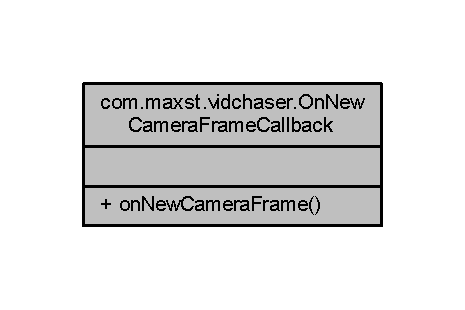
\includegraphics[width=223pt]{interfacecom_1_1maxst_1_1vidchaser_1_1_on_new_camera_frame_callback__coll__graph}
\end{center}
\end{figure}
\subsection*{Public Member Functions}
\begin{DoxyCompactItemize}
\item 
void \hyperlink{interfacecom_1_1maxst_1_1vidchaser_1_1_on_new_camera_frame_callback_ae69ef3264f4f6715f08b41ccec0dba76}{on\+New\+Camera\+Frame} (byte\mbox{[}$\,$\mbox{]} data, int length, int width, int height, int color\+Format)
\end{DoxyCompactItemize}


\subsection{Detailed Description}
Created by Jack on 2017-\/05-\/14. 

\subsection{Member Function Documentation}
\mbox{\Hypertarget{interfacecom_1_1maxst_1_1vidchaser_1_1_on_new_camera_frame_callback_ae69ef3264f4f6715f08b41ccec0dba76}\label{interfacecom_1_1maxst_1_1vidchaser_1_1_on_new_camera_frame_callback_ae69ef3264f4f6715f08b41ccec0dba76}} 
\index{com\+::maxst\+::vidchaser\+::\+On\+New\+Camera\+Frame\+Callback@{com\+::maxst\+::vidchaser\+::\+On\+New\+Camera\+Frame\+Callback}!on\+New\+Camera\+Frame@{on\+New\+Camera\+Frame}}
\index{on\+New\+Camera\+Frame@{on\+New\+Camera\+Frame}!com\+::maxst\+::vidchaser\+::\+On\+New\+Camera\+Frame\+Callback@{com\+::maxst\+::vidchaser\+::\+On\+New\+Camera\+Frame\+Callback}}
\subsubsection{\texorpdfstring{on\+New\+Camera\+Frame()}{onNewCameraFrame()}}
{\footnotesize\ttfamily void com.\+maxst.\+vidchaser.\+On\+New\+Camera\+Frame\+Callback.\+on\+New\+Camera\+Frame (\begin{DoxyParamCaption}\item[{byte \mbox{[}$\,$\mbox{]}}]{data,  }\item[{int}]{length,  }\item[{int}]{width,  }\item[{int}]{height,  }\item[{int}]{color\+Format }\end{DoxyParamCaption})}



The documentation for this interface was generated from the following file\+:\begin{DoxyCompactItemize}
\item 
C\+:/\+Workspace/\+Vid\+Chaser/\+Platform/\+Vid\+Chaser\+Android/\+Vid\+Chaser/src/main/java/com/maxst/vidchaser/\hyperlink{_on_new_camera_frame_callback_8java}{On\+New\+Camera\+Frame\+Callback.\+java}\end{DoxyCompactItemize}

\hypertarget{classcom_1_1maxst_1_1vidchaser_1_1_projection_matrix}{}\section{com.\+maxst.\+vidchaser.\+Projection\+Matrix Class Reference}
\label{classcom_1_1maxst_1_1vidchaser_1_1_projection_matrix}\index{com.\+maxst.\+vidchaser.\+Projection\+Matrix@{com.\+maxst.\+vidchaser.\+Projection\+Matrix}}


Collaboration diagram for com.\+maxst.\+vidchaser.\+Projection\+Matrix\+:\nopagebreak
\begin{figure}[H]
\begin{center}
\leavevmode
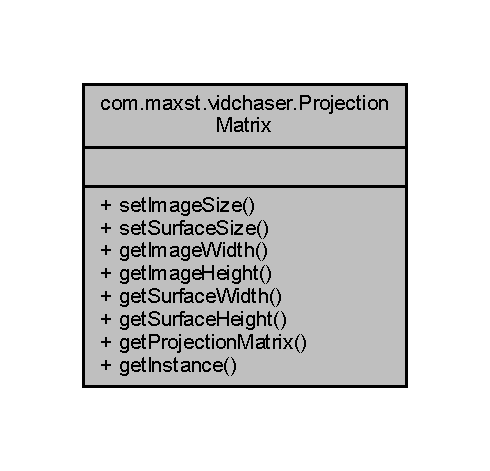
\includegraphics[width=235pt]{classcom_1_1maxst_1_1vidchaser_1_1_projection_matrix__coll__graph}
\end{center}
\end{figure}
\subsection*{Public Member Functions}
\begin{DoxyCompactItemize}
\item 
void \hyperlink{classcom_1_1maxst_1_1vidchaser_1_1_projection_matrix_ae450d0b28bfdb52b38989da684a9d29e}{set\+Image\+Size} (int width, int height)
\item 
void \hyperlink{classcom_1_1maxst_1_1vidchaser_1_1_projection_matrix_a64bdf3583a8aede82bb6fc6721346134}{set\+Surface\+Size} (int width, int height)
\item 
int \hyperlink{classcom_1_1maxst_1_1vidchaser_1_1_projection_matrix_a1e07354294afffdb44a61c7b7659e1fa}{get\+Image\+Width} ()
\item 
int \hyperlink{classcom_1_1maxst_1_1vidchaser_1_1_projection_matrix_a72e65465d3d38d1ef4f6bf187e72bf71}{get\+Image\+Height} ()
\item 
int \hyperlink{classcom_1_1maxst_1_1vidchaser_1_1_projection_matrix_a38b58ba2ddfd831dc86e6e92fb2fde10}{get\+Surface\+Width} ()
\item 
int \hyperlink{classcom_1_1maxst_1_1vidchaser_1_1_projection_matrix_a5db288183b110be0e8e403d90eed4a74}{get\+Surface\+Height} ()
\item 
float \mbox{[}$\,$\mbox{]} \hyperlink{classcom_1_1maxst_1_1vidchaser_1_1_projection_matrix_adddc52ee86b60d61eafbcca0bedc9386}{get\+Projection\+Matrix} ()
\end{DoxyCompactItemize}
\subsection*{Static Public Member Functions}
\begin{DoxyCompactItemize}
\item 
static \hyperlink{classcom_1_1maxst_1_1vidchaser_1_1_projection_matrix}{Projection\+Matrix} \hyperlink{classcom_1_1maxst_1_1vidchaser_1_1_projection_matrix_afb7c50dffd1d73e23680af04b5ba5a04}{get\+Instance} ()
\end{DoxyCompactItemize}


\subsection{Member Function Documentation}
\mbox{\Hypertarget{classcom_1_1maxst_1_1vidchaser_1_1_projection_matrix_a72e65465d3d38d1ef4f6bf187e72bf71}\label{classcom_1_1maxst_1_1vidchaser_1_1_projection_matrix_a72e65465d3d38d1ef4f6bf187e72bf71}} 
\index{com\+::maxst\+::vidchaser\+::\+Projection\+Matrix@{com\+::maxst\+::vidchaser\+::\+Projection\+Matrix}!get\+Image\+Height@{get\+Image\+Height}}
\index{get\+Image\+Height@{get\+Image\+Height}!com\+::maxst\+::vidchaser\+::\+Projection\+Matrix@{com\+::maxst\+::vidchaser\+::\+Projection\+Matrix}}
\subsubsection{\texorpdfstring{get\+Image\+Height()}{getImageHeight()}}
{\footnotesize\ttfamily int com.\+maxst.\+vidchaser.\+Projection\+Matrix.\+get\+Image\+Height (\begin{DoxyParamCaption}{ }\end{DoxyParamCaption})}

Here is the caller graph for this function\+:\nopagebreak
\begin{figure}[H]
\begin{center}
\leavevmode
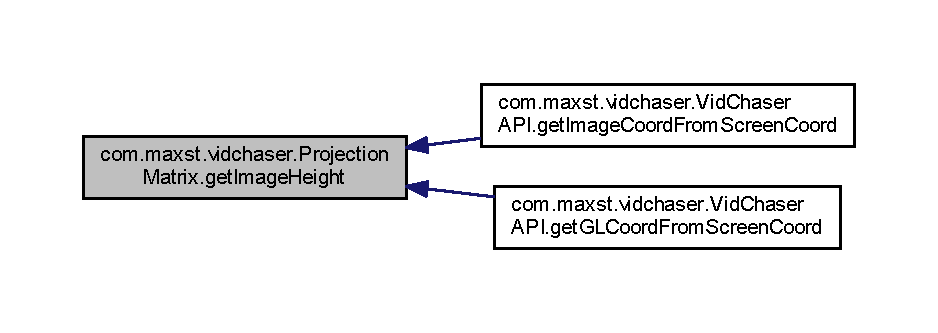
\includegraphics[width=350pt]{classcom_1_1maxst_1_1vidchaser_1_1_projection_matrix_a72e65465d3d38d1ef4f6bf187e72bf71_icgraph}
\end{center}
\end{figure}
\mbox{\Hypertarget{classcom_1_1maxst_1_1vidchaser_1_1_projection_matrix_a1e07354294afffdb44a61c7b7659e1fa}\label{classcom_1_1maxst_1_1vidchaser_1_1_projection_matrix_a1e07354294afffdb44a61c7b7659e1fa}} 
\index{com\+::maxst\+::vidchaser\+::\+Projection\+Matrix@{com\+::maxst\+::vidchaser\+::\+Projection\+Matrix}!get\+Image\+Width@{get\+Image\+Width}}
\index{get\+Image\+Width@{get\+Image\+Width}!com\+::maxst\+::vidchaser\+::\+Projection\+Matrix@{com\+::maxst\+::vidchaser\+::\+Projection\+Matrix}}
\subsubsection{\texorpdfstring{get\+Image\+Width()}{getImageWidth()}}
{\footnotesize\ttfamily int com.\+maxst.\+vidchaser.\+Projection\+Matrix.\+get\+Image\+Width (\begin{DoxyParamCaption}{ }\end{DoxyParamCaption})}

Here is the caller graph for this function\+:\nopagebreak
\begin{figure}[H]
\begin{center}
\leavevmode
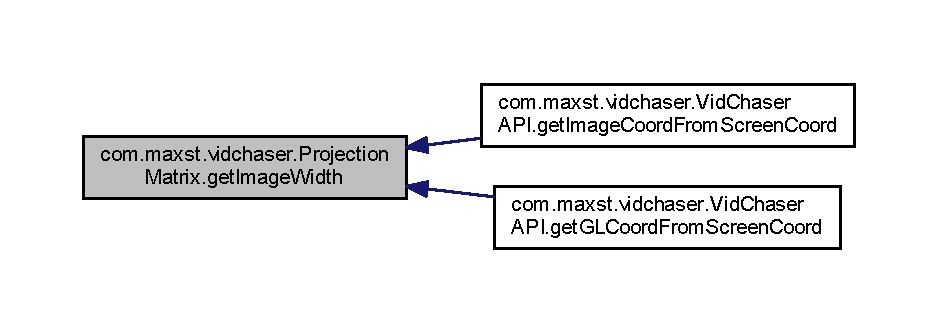
\includegraphics[width=350pt]{classcom_1_1maxst_1_1vidchaser_1_1_projection_matrix_a1e07354294afffdb44a61c7b7659e1fa_icgraph}
\end{center}
\end{figure}
\mbox{\Hypertarget{classcom_1_1maxst_1_1vidchaser_1_1_projection_matrix_afb7c50dffd1d73e23680af04b5ba5a04}\label{classcom_1_1maxst_1_1vidchaser_1_1_projection_matrix_afb7c50dffd1d73e23680af04b5ba5a04}} 
\index{com\+::maxst\+::vidchaser\+::\+Projection\+Matrix@{com\+::maxst\+::vidchaser\+::\+Projection\+Matrix}!get\+Instance@{get\+Instance}}
\index{get\+Instance@{get\+Instance}!com\+::maxst\+::vidchaser\+::\+Projection\+Matrix@{com\+::maxst\+::vidchaser\+::\+Projection\+Matrix}}
\subsubsection{\texorpdfstring{get\+Instance()}{getInstance()}}
{\footnotesize\ttfamily static \hyperlink{classcom_1_1maxst_1_1vidchaser_1_1_projection_matrix}{Projection\+Matrix} com.\+maxst.\+vidchaser.\+Projection\+Matrix.\+get\+Instance (\begin{DoxyParamCaption}{ }\end{DoxyParamCaption})\hspace{0.3cm}{\ttfamily [static]}}

Here is the caller graph for this function\+:\nopagebreak
\begin{figure}[H]
\begin{center}
\leavevmode
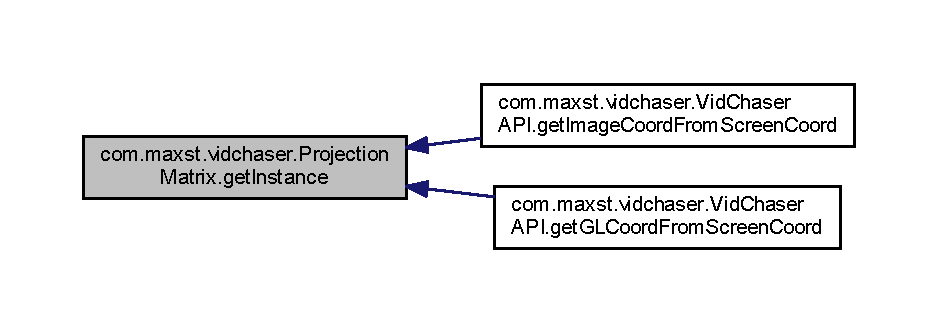
\includegraphics[width=350pt]{classcom_1_1maxst_1_1vidchaser_1_1_projection_matrix_afb7c50dffd1d73e23680af04b5ba5a04_icgraph}
\end{center}
\end{figure}
\mbox{\Hypertarget{classcom_1_1maxst_1_1vidchaser_1_1_projection_matrix_adddc52ee86b60d61eafbcca0bedc9386}\label{classcom_1_1maxst_1_1vidchaser_1_1_projection_matrix_adddc52ee86b60d61eafbcca0bedc9386}} 
\index{com\+::maxst\+::vidchaser\+::\+Projection\+Matrix@{com\+::maxst\+::vidchaser\+::\+Projection\+Matrix}!get\+Projection\+Matrix@{get\+Projection\+Matrix}}
\index{get\+Projection\+Matrix@{get\+Projection\+Matrix}!com\+::maxst\+::vidchaser\+::\+Projection\+Matrix@{com\+::maxst\+::vidchaser\+::\+Projection\+Matrix}}
\subsubsection{\texorpdfstring{get\+Projection\+Matrix()}{getProjectionMatrix()}}
{\footnotesize\ttfamily float \mbox{[}$\,$\mbox{]} com.\+maxst.\+vidchaser.\+Projection\+Matrix.\+get\+Projection\+Matrix (\begin{DoxyParamCaption}{ }\end{DoxyParamCaption})}

\mbox{\Hypertarget{classcom_1_1maxst_1_1vidchaser_1_1_projection_matrix_a5db288183b110be0e8e403d90eed4a74}\label{classcom_1_1maxst_1_1vidchaser_1_1_projection_matrix_a5db288183b110be0e8e403d90eed4a74}} 
\index{com\+::maxst\+::vidchaser\+::\+Projection\+Matrix@{com\+::maxst\+::vidchaser\+::\+Projection\+Matrix}!get\+Surface\+Height@{get\+Surface\+Height}}
\index{get\+Surface\+Height@{get\+Surface\+Height}!com\+::maxst\+::vidchaser\+::\+Projection\+Matrix@{com\+::maxst\+::vidchaser\+::\+Projection\+Matrix}}
\subsubsection{\texorpdfstring{get\+Surface\+Height()}{getSurfaceHeight()}}
{\footnotesize\ttfamily int com.\+maxst.\+vidchaser.\+Projection\+Matrix.\+get\+Surface\+Height (\begin{DoxyParamCaption}{ }\end{DoxyParamCaption})}

Here is the caller graph for this function\+:\nopagebreak
\begin{figure}[H]
\begin{center}
\leavevmode
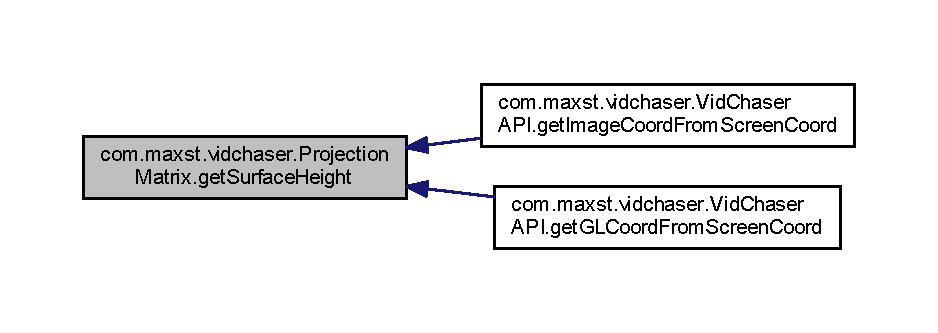
\includegraphics[width=350pt]{classcom_1_1maxst_1_1vidchaser_1_1_projection_matrix_a5db288183b110be0e8e403d90eed4a74_icgraph}
\end{center}
\end{figure}
\mbox{\Hypertarget{classcom_1_1maxst_1_1vidchaser_1_1_projection_matrix_a38b58ba2ddfd831dc86e6e92fb2fde10}\label{classcom_1_1maxst_1_1vidchaser_1_1_projection_matrix_a38b58ba2ddfd831dc86e6e92fb2fde10}} 
\index{com\+::maxst\+::vidchaser\+::\+Projection\+Matrix@{com\+::maxst\+::vidchaser\+::\+Projection\+Matrix}!get\+Surface\+Width@{get\+Surface\+Width}}
\index{get\+Surface\+Width@{get\+Surface\+Width}!com\+::maxst\+::vidchaser\+::\+Projection\+Matrix@{com\+::maxst\+::vidchaser\+::\+Projection\+Matrix}}
\subsubsection{\texorpdfstring{get\+Surface\+Width()}{getSurfaceWidth()}}
{\footnotesize\ttfamily int com.\+maxst.\+vidchaser.\+Projection\+Matrix.\+get\+Surface\+Width (\begin{DoxyParamCaption}{ }\end{DoxyParamCaption})}

Here is the caller graph for this function\+:\nopagebreak
\begin{figure}[H]
\begin{center}
\leavevmode
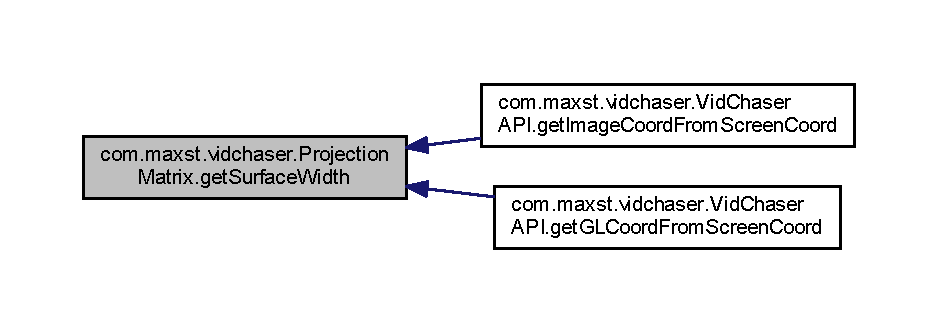
\includegraphics[width=350pt]{classcom_1_1maxst_1_1vidchaser_1_1_projection_matrix_a38b58ba2ddfd831dc86e6e92fb2fde10_icgraph}
\end{center}
\end{figure}
\mbox{\Hypertarget{classcom_1_1maxst_1_1vidchaser_1_1_projection_matrix_ae450d0b28bfdb52b38989da684a9d29e}\label{classcom_1_1maxst_1_1vidchaser_1_1_projection_matrix_ae450d0b28bfdb52b38989da684a9d29e}} 
\index{com\+::maxst\+::vidchaser\+::\+Projection\+Matrix@{com\+::maxst\+::vidchaser\+::\+Projection\+Matrix}!set\+Image\+Size@{set\+Image\+Size}}
\index{set\+Image\+Size@{set\+Image\+Size}!com\+::maxst\+::vidchaser\+::\+Projection\+Matrix@{com\+::maxst\+::vidchaser\+::\+Projection\+Matrix}}
\subsubsection{\texorpdfstring{set\+Image\+Size()}{setImageSize()}}
{\footnotesize\ttfamily void com.\+maxst.\+vidchaser.\+Projection\+Matrix.\+set\+Image\+Size (\begin{DoxyParamCaption}\item[{int}]{width,  }\item[{int}]{height }\end{DoxyParamCaption})}

\mbox{\Hypertarget{classcom_1_1maxst_1_1vidchaser_1_1_projection_matrix_a64bdf3583a8aede82bb6fc6721346134}\label{classcom_1_1maxst_1_1vidchaser_1_1_projection_matrix_a64bdf3583a8aede82bb6fc6721346134}} 
\index{com\+::maxst\+::vidchaser\+::\+Projection\+Matrix@{com\+::maxst\+::vidchaser\+::\+Projection\+Matrix}!set\+Surface\+Size@{set\+Surface\+Size}}
\index{set\+Surface\+Size@{set\+Surface\+Size}!com\+::maxst\+::vidchaser\+::\+Projection\+Matrix@{com\+::maxst\+::vidchaser\+::\+Projection\+Matrix}}
\subsubsection{\texorpdfstring{set\+Surface\+Size()}{setSurfaceSize()}}
{\footnotesize\ttfamily void com.\+maxst.\+vidchaser.\+Projection\+Matrix.\+set\+Surface\+Size (\begin{DoxyParamCaption}\item[{int}]{width,  }\item[{int}]{height }\end{DoxyParamCaption})}



The documentation for this class was generated from the following file\+:\begin{DoxyCompactItemize}
\item 
C\+:/\+Workspace/\+Vid\+Chaser/\+Platform/\+Vid\+Chaser\+Android/\+Vid\+Chaser/src/main/java/com/maxst/vidchaser/\hyperlink{_projection_matrix_8java}{Projection\+Matrix.\+java}\end{DoxyCompactItemize}

\hypertarget{classcom_1_1maxst_1_1vidchaser_1_1_vid_chaser_a_p_i}{}\section{com.\+maxst.\+vidchaser.\+Vid\+Chaser\+A\+PI Class Reference}
\label{classcom_1_1maxst_1_1vidchaser_1_1_vid_chaser_a_p_i}\index{com.\+maxst.\+vidchaser.\+Vid\+Chaser\+A\+PI@{com.\+maxst.\+vidchaser.\+Vid\+Chaser\+A\+PI}}


Collaboration diagram for com.\+maxst.\+vidchaser.\+Vid\+Chaser\+A\+PI\+:\nopagebreak
\begin{figure}[H]
\begin{center}
\leavevmode
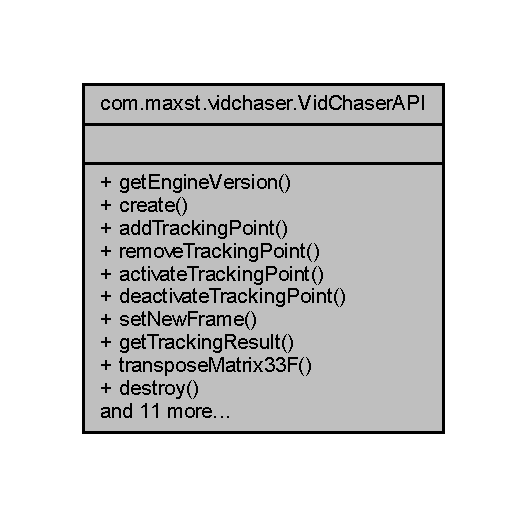
\includegraphics[width=253pt]{classcom_1_1maxst_1_1vidchaser_1_1_vid_chaser_a_p_i__coll__graph}
\end{center}
\end{figure}
\subsection*{Static Public Member Functions}
\begin{DoxyCompactItemize}
\item 
static String \hyperlink{classcom_1_1maxst_1_1vidchaser_1_1_vid_chaser_a_p_i_a0a384a71903aca04dad7ae5a7b641da9}{get\+Engine\+Version} ()
\item 
static int \hyperlink{classcom_1_1maxst_1_1vidchaser_1_1_vid_chaser_a_p_i_aa9a6cbc276431f56d11509c22c640749}{create} (Context context, String app\+Key)
\item 
static int \hyperlink{classcom_1_1maxst_1_1vidchaser_1_1_vid_chaser_a_p_i_a39767b1ffd8a00d529d3183a00dd45b3}{add\+Tracking\+Point} (int imageX, int imageY, int \mbox{[}$\,$\mbox{]} trackable\+Id, int tracking\+Method)
\item 
static int \hyperlink{classcom_1_1maxst_1_1vidchaser_1_1_vid_chaser_a_p_i_a52b3b148426377d86b7e3985ca4625fe}{remove\+Tracking\+Point} (int trackable\+Id)
\item 
static int \hyperlink{classcom_1_1maxst_1_1vidchaser_1_1_vid_chaser_a_p_i_a70d462cf63aa4c014a0cc42f3af9f3d4}{activate\+Tracking\+Point} (int imageX, int imageY, int index)
\begin{DoxyCompactList}\small\item\em activate tracking point(index) \end{DoxyCompactList}\item 
static int \hyperlink{classcom_1_1maxst_1_1vidchaser_1_1_vid_chaser_a_p_i_a36952cb46625a4a4ee0fa7183fbf03b1}{deactivate\+Tracking\+Point} (int index)
\begin{DoxyCompactList}\small\item\em deactivate tracking point(index) \end{DoxyCompactList}\item 
static int \hyperlink{classcom_1_1maxst_1_1vidchaser_1_1_vid_chaser_a_p_i_af391e17e712749adbb5bfee2b762d941}{set\+New\+Frame} (byte\mbox{[}$\,$\mbox{]} image\+Data, int start\+Offset, int length, int image\+Width, int image\+Height, int stride, int image\+Format, int image\+Index)
\item 
static int \hyperlink{classcom_1_1maxst_1_1vidchaser_1_1_vid_chaser_a_p_i_aa7555cd0125d9d7e3c2d3eae519ce1b0}{get\+Tracking\+Result} (float \mbox{[}$\,$\mbox{]} result, int trackable\+Id, int\mbox{[}$\,$\mbox{]} process\+Time)
\item 
static void \hyperlink{classcom_1_1maxst_1_1vidchaser_1_1_vid_chaser_a_p_i_a7883ba1837bd5c3f84ec45ca66414b05}{transpose\+Matrix33F} (float \mbox{[}$\,$\mbox{]} in, float \mbox{[}$\,$\mbox{]} out)
\item 
static int \hyperlink{classcom_1_1maxst_1_1vidchaser_1_1_vid_chaser_a_p_i_a89080c8433fe0a5361f5ca660908b183}{destroy} ()
\item 
static void \hyperlink{classcom_1_1maxst_1_1vidchaser_1_1_vid_chaser_a_p_i_ad862cc3057d072216e0f3a7b4e9e295b}{get\+Image\+Coord\+From\+Screen\+Coord} (int screenX, int screenY, int\mbox{[}$\,$\mbox{]} image\+Coord)
\item 
static void \hyperlink{classcom_1_1maxst_1_1vidchaser_1_1_vid_chaser_a_p_i_a023777164b60f04666b2e5b718580e03}{get\+G\+L\+Coord\+From\+Screen\+Coord} (int screenX, int screenY, float\mbox{[}$\,$\mbox{]} gl\+Coord)
\item 
static void \hyperlink{classcom_1_1maxst_1_1vidchaser_1_1_vid_chaser_a_p_i_a289c720643c1f900f956f2589a619871}{get\+Transform\+Matrix44F} (int image\+Width, int image\+Height, float\mbox{[}$\,$\mbox{]} transform\+Matrix33F, float\mbox{[}$\,$\mbox{]} transform\+Matrix44F)
\item 
static void \hyperlink{classcom_1_1maxst_1_1vidchaser_1_1_vid_chaser_a_p_i_a89cea03eb38771648663da04950aaec5}{set\+On\+New\+Camera\+Frame\+Callback} (\hyperlink{interfacecom_1_1maxst_1_1vidchaser_1_1_on_new_camera_frame_callback}{On\+New\+Camera\+Frame\+Callback} callback)
\item 
static void \hyperlink{classcom_1_1maxst_1_1vidchaser_1_1_vid_chaser_a_p_i_a80334a0ee1380fddc6a469facee88492}{save\+Camera\+Frame} (String file\+Name, byte \mbox{[}$\,$\mbox{]} data, int length, int width, int height, int stride, int save\+Color\+Format)
\item 
static void \hyperlink{classcom_1_1maxst_1_1vidchaser_1_1_vid_chaser_a_p_i_ab4f43383db7d47da64c1c2b9ab8167ac}{start\+Camera} (int camera\+Id, int width, int height)
\item 
static void \hyperlink{classcom_1_1maxst_1_1vidchaser_1_1_vid_chaser_a_p_i_af7092d1f3dcca228cb6a45f263e35120}{stop\+Camera} ()
\item 
static void \hyperlink{classcom_1_1maxst_1_1vidchaser_1_1_vid_chaser_a_p_i_af4e7ca30f3836348d7f5a2b375a25d28}{init\+Redering} ()
\item 
static void \hyperlink{classcom_1_1maxst_1_1vidchaser_1_1_vid_chaser_a_p_i_a72fa4502f5dcc8d1e765167be9a05cae}{update\+Rendering} (int width, int height)
\item 
static void \hyperlink{classcom_1_1maxst_1_1vidchaser_1_1_vid_chaser_a_p_i_a8a695391dde4caec8e85e5355769e202}{render\+Scene} ()
\item 
static void \hyperlink{classcom_1_1maxst_1_1vidchaser_1_1_vid_chaser_a_p_i_ab9d7cb7188771fac801aa2e9aefc6a83}{deinit\+Rendering} ()
\end{DoxyCompactItemize}


\subsection{Member Function Documentation}
\mbox{\Hypertarget{classcom_1_1maxst_1_1vidchaser_1_1_vid_chaser_a_p_i_a70d462cf63aa4c014a0cc42f3af9f3d4}\label{classcom_1_1maxst_1_1vidchaser_1_1_vid_chaser_a_p_i_a70d462cf63aa4c014a0cc42f3af9f3d4}} 
\index{com\+::maxst\+::vidchaser\+::\+Vid\+Chaser\+A\+PI@{com\+::maxst\+::vidchaser\+::\+Vid\+Chaser\+A\+PI}!activate\+Tracking\+Point@{activate\+Tracking\+Point}}
\index{activate\+Tracking\+Point@{activate\+Tracking\+Point}!com\+::maxst\+::vidchaser\+::\+Vid\+Chaser\+A\+PI@{com\+::maxst\+::vidchaser\+::\+Vid\+Chaser\+A\+PI}}
\subsubsection{\texorpdfstring{activate\+Tracking\+Point()}{activateTrackingPoint()}}
{\footnotesize\ttfamily static int com.\+maxst.\+vidchaser.\+Vid\+Chaser\+A\+P\+I.\+activate\+Tracking\+Point (\begin{DoxyParamCaption}\item[{int}]{imageX,  }\item[{int}]{imageY,  }\item[{int}]{index }\end{DoxyParamCaption})\hspace{0.3cm}{\ttfamily [static]}}



activate tracking point(index) 


\begin{DoxyParams}{Parameters}
{\em imageX} & reset tracking position x(pixel). \\
\hline
{\em imageY} & reset tracking position y(pixel). \\
\hline
{\em index} & tracking point index that will be changed status. return result code. \\
\hline
\end{DoxyParams}
\mbox{\Hypertarget{classcom_1_1maxst_1_1vidchaser_1_1_vid_chaser_a_p_i_a39767b1ffd8a00d529d3183a00dd45b3}\label{classcom_1_1maxst_1_1vidchaser_1_1_vid_chaser_a_p_i_a39767b1ffd8a00d529d3183a00dd45b3}} 
\index{com\+::maxst\+::vidchaser\+::\+Vid\+Chaser\+A\+PI@{com\+::maxst\+::vidchaser\+::\+Vid\+Chaser\+A\+PI}!add\+Tracking\+Point@{add\+Tracking\+Point}}
\index{add\+Tracking\+Point@{add\+Tracking\+Point}!com\+::maxst\+::vidchaser\+::\+Vid\+Chaser\+A\+PI@{com\+::maxst\+::vidchaser\+::\+Vid\+Chaser\+A\+PI}}
\subsubsection{\texorpdfstring{add\+Tracking\+Point()}{addTrackingPoint()}}
{\footnotesize\ttfamily static int com.\+maxst.\+vidchaser.\+Vid\+Chaser\+A\+P\+I.\+add\+Tracking\+Point (\begin{DoxyParamCaption}\item[{int}]{imageX,  }\item[{int}]{imageY,  }\item[{int \mbox{[}$\,$\mbox{]}}]{trackable\+Id,  }\item[{int}]{tracking\+Method }\end{DoxyParamCaption})\hspace{0.3cm}{\ttfamily [static]}}

Add tracking point on Image coordinate.


\begin{DoxyParams}{Parameters}
{\em imageX} & X position on Image coordinate \\
\hline
{\em imageY} & Y position on Image coordinate \\
\hline
{\em trackable\+Id} & trackable\+Id container which is created by Vid\+Chaser engine \\
\hline
{\em tracking\+Method} & Tracking method index \\
\hline
\end{DoxyParams}
\begin{DoxyReturn}{Returns}
Return result code 
\end{DoxyReturn}
\mbox{\Hypertarget{classcom_1_1maxst_1_1vidchaser_1_1_vid_chaser_a_p_i_aa9a6cbc276431f56d11509c22c640749}\label{classcom_1_1maxst_1_1vidchaser_1_1_vid_chaser_a_p_i_aa9a6cbc276431f56d11509c22c640749}} 
\index{com\+::maxst\+::vidchaser\+::\+Vid\+Chaser\+A\+PI@{com\+::maxst\+::vidchaser\+::\+Vid\+Chaser\+A\+PI}!create@{create}}
\index{create@{create}!com\+::maxst\+::vidchaser\+::\+Vid\+Chaser\+A\+PI@{com\+::maxst\+::vidchaser\+::\+Vid\+Chaser\+A\+PI}}
\subsubsection{\texorpdfstring{create()}{create()}}
{\footnotesize\ttfamily static int com.\+maxst.\+vidchaser.\+Vid\+Chaser\+A\+P\+I.\+create (\begin{DoxyParamCaption}\item[{Context}]{context,  }\item[{String}]{app\+Key }\end{DoxyParamCaption})\hspace{0.3cm}{\ttfamily [static]}}

Initialize tracker.


\begin{DoxyParams}{Parameters}
{\em context} & Application context \\
\hline
{\em app\+Key} & App license key \\
\hline
\end{DoxyParams}
\begin{DoxyReturn}{Returns}
Return result code 
\end{DoxyReturn}
\mbox{\Hypertarget{classcom_1_1maxst_1_1vidchaser_1_1_vid_chaser_a_p_i_a36952cb46625a4a4ee0fa7183fbf03b1}\label{classcom_1_1maxst_1_1vidchaser_1_1_vid_chaser_a_p_i_a36952cb46625a4a4ee0fa7183fbf03b1}} 
\index{com\+::maxst\+::vidchaser\+::\+Vid\+Chaser\+A\+PI@{com\+::maxst\+::vidchaser\+::\+Vid\+Chaser\+A\+PI}!deactivate\+Tracking\+Point@{deactivate\+Tracking\+Point}}
\index{deactivate\+Tracking\+Point@{deactivate\+Tracking\+Point}!com\+::maxst\+::vidchaser\+::\+Vid\+Chaser\+A\+PI@{com\+::maxst\+::vidchaser\+::\+Vid\+Chaser\+A\+PI}}
\subsubsection{\texorpdfstring{deactivate\+Tracking\+Point()}{deactivateTrackingPoint()}}
{\footnotesize\ttfamily static int com.\+maxst.\+vidchaser.\+Vid\+Chaser\+A\+P\+I.\+deactivate\+Tracking\+Point (\begin{DoxyParamCaption}\item[{int}]{index }\end{DoxyParamCaption})\hspace{0.3cm}{\ttfamily [static]}}



deactivate tracking point(index) 


\begin{DoxyParams}{Parameters}
{\em index} & tracking point index that will be changed status. return result code. \\
\hline
\end{DoxyParams}
\mbox{\Hypertarget{classcom_1_1maxst_1_1vidchaser_1_1_vid_chaser_a_p_i_ab9d7cb7188771fac801aa2e9aefc6a83}\label{classcom_1_1maxst_1_1vidchaser_1_1_vid_chaser_a_p_i_ab9d7cb7188771fac801aa2e9aefc6a83}} 
\index{com\+::maxst\+::vidchaser\+::\+Vid\+Chaser\+A\+PI@{com\+::maxst\+::vidchaser\+::\+Vid\+Chaser\+A\+PI}!deinit\+Rendering@{deinit\+Rendering}}
\index{deinit\+Rendering@{deinit\+Rendering}!com\+::maxst\+::vidchaser\+::\+Vid\+Chaser\+A\+PI@{com\+::maxst\+::vidchaser\+::\+Vid\+Chaser\+A\+PI}}
\subsubsection{\texorpdfstring{deinit\+Rendering()}{deinitRendering()}}
{\footnotesize\ttfamily static void com.\+maxst.\+vidchaser.\+Vid\+Chaser\+A\+P\+I.\+deinit\+Rendering (\begin{DoxyParamCaption}{ }\end{DoxyParamCaption})\hspace{0.3cm}{\ttfamily [static]}}

\mbox{\Hypertarget{classcom_1_1maxst_1_1vidchaser_1_1_vid_chaser_a_p_i_a89080c8433fe0a5361f5ca660908b183}\label{classcom_1_1maxst_1_1vidchaser_1_1_vid_chaser_a_p_i_a89080c8433fe0a5361f5ca660908b183}} 
\index{com\+::maxst\+::vidchaser\+::\+Vid\+Chaser\+A\+PI@{com\+::maxst\+::vidchaser\+::\+Vid\+Chaser\+A\+PI}!destroy@{destroy}}
\index{destroy@{destroy}!com\+::maxst\+::vidchaser\+::\+Vid\+Chaser\+A\+PI@{com\+::maxst\+::vidchaser\+::\+Vid\+Chaser\+A\+PI}}
\subsubsection{\texorpdfstring{destroy()}{destroy()}}
{\footnotesize\ttfamily static int com.\+maxst.\+vidchaser.\+Vid\+Chaser\+A\+P\+I.\+destroy (\begin{DoxyParamCaption}{ }\end{DoxyParamCaption})\hspace{0.3cm}{\ttfamily [static]}}

Destroy tracker engine. \begin{DoxyReturn}{Returns}
Return result code 
\end{DoxyReturn}
\mbox{\Hypertarget{classcom_1_1maxst_1_1vidchaser_1_1_vid_chaser_a_p_i_a0a384a71903aca04dad7ae5a7b641da9}\label{classcom_1_1maxst_1_1vidchaser_1_1_vid_chaser_a_p_i_a0a384a71903aca04dad7ae5a7b641da9}} 
\index{com\+::maxst\+::vidchaser\+::\+Vid\+Chaser\+A\+PI@{com\+::maxst\+::vidchaser\+::\+Vid\+Chaser\+A\+PI}!get\+Engine\+Version@{get\+Engine\+Version}}
\index{get\+Engine\+Version@{get\+Engine\+Version}!com\+::maxst\+::vidchaser\+::\+Vid\+Chaser\+A\+PI@{com\+::maxst\+::vidchaser\+::\+Vid\+Chaser\+A\+PI}}
\subsubsection{\texorpdfstring{get\+Engine\+Version()}{getEngineVersion()}}
{\footnotesize\ttfamily static String com.\+maxst.\+vidchaser.\+Vid\+Chaser\+A\+P\+I.\+get\+Engine\+Version (\begin{DoxyParamCaption}{ }\end{DoxyParamCaption})\hspace{0.3cm}{\ttfamily [static]}}

Get tracker version.

\begin{DoxyReturn}{Returns}
Engine version. 
\end{DoxyReturn}
\mbox{\Hypertarget{classcom_1_1maxst_1_1vidchaser_1_1_vid_chaser_a_p_i_a023777164b60f04666b2e5b718580e03}\label{classcom_1_1maxst_1_1vidchaser_1_1_vid_chaser_a_p_i_a023777164b60f04666b2e5b718580e03}} 
\index{com\+::maxst\+::vidchaser\+::\+Vid\+Chaser\+A\+PI@{com\+::maxst\+::vidchaser\+::\+Vid\+Chaser\+A\+PI}!get\+G\+L\+Coord\+From\+Screen\+Coord@{get\+G\+L\+Coord\+From\+Screen\+Coord}}
\index{get\+G\+L\+Coord\+From\+Screen\+Coord@{get\+G\+L\+Coord\+From\+Screen\+Coord}!com\+::maxst\+::vidchaser\+::\+Vid\+Chaser\+A\+PI@{com\+::maxst\+::vidchaser\+::\+Vid\+Chaser\+A\+PI}}
\subsubsection{\texorpdfstring{get\+G\+L\+Coord\+From\+Screen\+Coord()}{getGLCoordFromScreenCoord()}}
{\footnotesize\ttfamily static void com.\+maxst.\+vidchaser.\+Vid\+Chaser\+A\+P\+I.\+get\+G\+L\+Coord\+From\+Screen\+Coord (\begin{DoxyParamCaption}\item[{int}]{screenX,  }\item[{int}]{screenY,  }\item[{float \mbox{[}$\,$\mbox{]}}]{gl\+Coord }\end{DoxyParamCaption})\hspace{0.3cm}{\ttfamily [static]}}

Here is the call graph for this function\+:\nopagebreak
\begin{figure}[H]
\begin{center}
\leavevmode
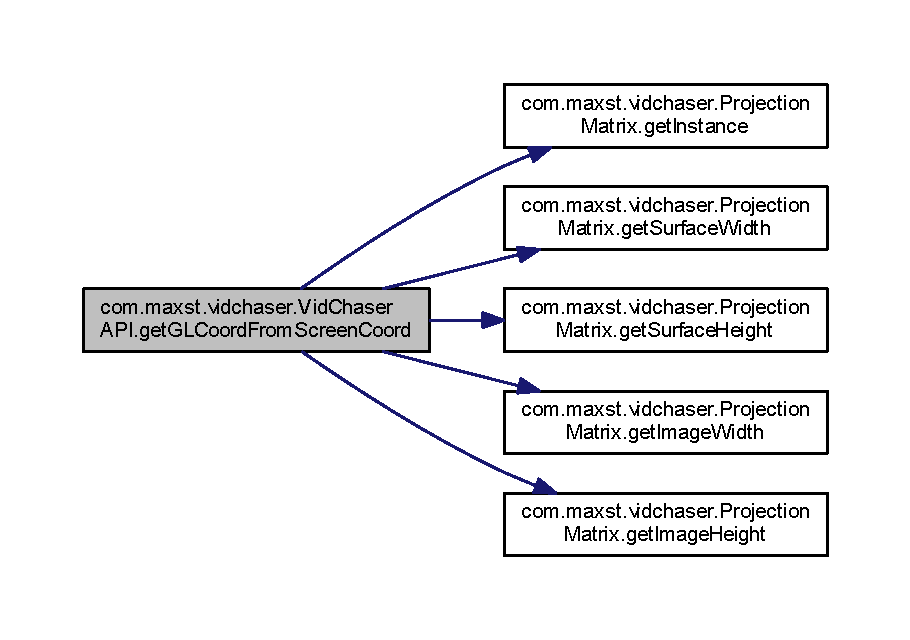
\includegraphics[width=350pt]{classcom_1_1maxst_1_1vidchaser_1_1_vid_chaser_a_p_i_a023777164b60f04666b2e5b718580e03_cgraph}
\end{center}
\end{figure}
\mbox{\Hypertarget{classcom_1_1maxst_1_1vidchaser_1_1_vid_chaser_a_p_i_ad862cc3057d072216e0f3a7b4e9e295b}\label{classcom_1_1maxst_1_1vidchaser_1_1_vid_chaser_a_p_i_ad862cc3057d072216e0f3a7b4e9e295b}} 
\index{com\+::maxst\+::vidchaser\+::\+Vid\+Chaser\+A\+PI@{com\+::maxst\+::vidchaser\+::\+Vid\+Chaser\+A\+PI}!get\+Image\+Coord\+From\+Screen\+Coord@{get\+Image\+Coord\+From\+Screen\+Coord}}
\index{get\+Image\+Coord\+From\+Screen\+Coord@{get\+Image\+Coord\+From\+Screen\+Coord}!com\+::maxst\+::vidchaser\+::\+Vid\+Chaser\+A\+PI@{com\+::maxst\+::vidchaser\+::\+Vid\+Chaser\+A\+PI}}
\subsubsection{\texorpdfstring{get\+Image\+Coord\+From\+Screen\+Coord()}{getImageCoordFromScreenCoord()}}
{\footnotesize\ttfamily static void com.\+maxst.\+vidchaser.\+Vid\+Chaser\+A\+P\+I.\+get\+Image\+Coord\+From\+Screen\+Coord (\begin{DoxyParamCaption}\item[{int}]{screenX,  }\item[{int}]{screenY,  }\item[{int \mbox{[}$\,$\mbox{]}}]{image\+Coord }\end{DoxyParamCaption})\hspace{0.3cm}{\ttfamily [static]}}

Here is the call graph for this function\+:\nopagebreak
\begin{figure}[H]
\begin{center}
\leavevmode
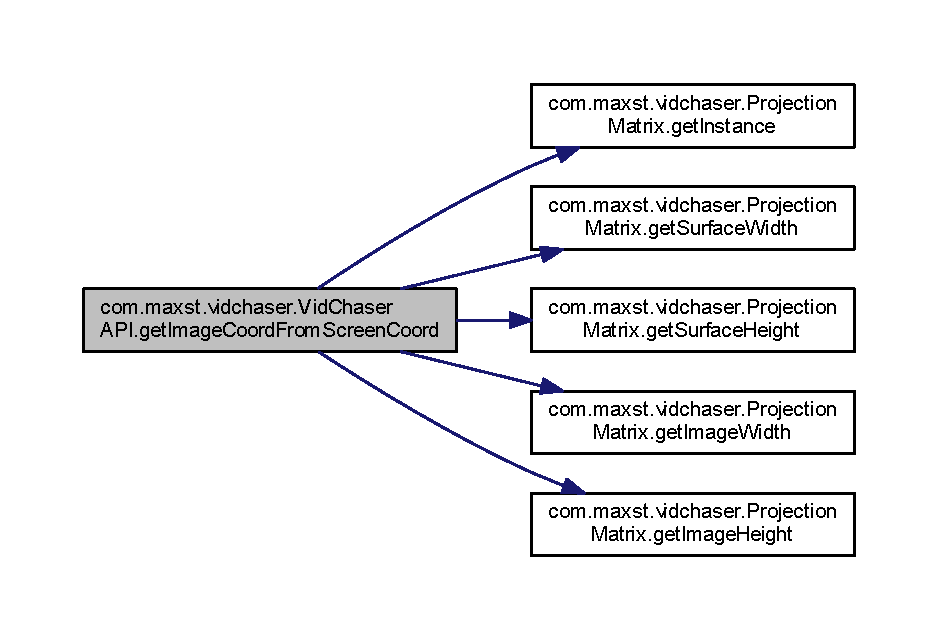
\includegraphics[width=350pt]{classcom_1_1maxst_1_1vidchaser_1_1_vid_chaser_a_p_i_ad862cc3057d072216e0f3a7b4e9e295b_cgraph}
\end{center}
\end{figure}
\mbox{\Hypertarget{classcom_1_1maxst_1_1vidchaser_1_1_vid_chaser_a_p_i_aa7555cd0125d9d7e3c2d3eae519ce1b0}\label{classcom_1_1maxst_1_1vidchaser_1_1_vid_chaser_a_p_i_aa7555cd0125d9d7e3c2d3eae519ce1b0}} 
\index{com\+::maxst\+::vidchaser\+::\+Vid\+Chaser\+A\+PI@{com\+::maxst\+::vidchaser\+::\+Vid\+Chaser\+A\+PI}!get\+Tracking\+Result@{get\+Tracking\+Result}}
\index{get\+Tracking\+Result@{get\+Tracking\+Result}!com\+::maxst\+::vidchaser\+::\+Vid\+Chaser\+A\+PI@{com\+::maxst\+::vidchaser\+::\+Vid\+Chaser\+A\+PI}}
\subsubsection{\texorpdfstring{get\+Tracking\+Result()}{getTrackingResult()}}
{\footnotesize\ttfamily static int com.\+maxst.\+vidchaser.\+Vid\+Chaser\+A\+P\+I.\+get\+Tracking\+Result (\begin{DoxyParamCaption}\item[{float \mbox{[}$\,$\mbox{]}}]{result,  }\item[{int}]{trackable\+Id,  }\item[{int \mbox{[}$\,$\mbox{]}}]{process\+Time }\end{DoxyParamCaption})\hspace{0.3cm}{\ttfamily [static]}}

\mbox{\Hypertarget{classcom_1_1maxst_1_1vidchaser_1_1_vid_chaser_a_p_i_a289c720643c1f900f956f2589a619871}\label{classcom_1_1maxst_1_1vidchaser_1_1_vid_chaser_a_p_i_a289c720643c1f900f956f2589a619871}} 
\index{com\+::maxst\+::vidchaser\+::\+Vid\+Chaser\+A\+PI@{com\+::maxst\+::vidchaser\+::\+Vid\+Chaser\+A\+PI}!get\+Transform\+Matrix44F@{get\+Transform\+Matrix44F}}
\index{get\+Transform\+Matrix44F@{get\+Transform\+Matrix44F}!com\+::maxst\+::vidchaser\+::\+Vid\+Chaser\+A\+PI@{com\+::maxst\+::vidchaser\+::\+Vid\+Chaser\+A\+PI}}
\subsubsection{\texorpdfstring{get\+Transform\+Matrix44\+F()}{getTransformMatrix44F()}}
{\footnotesize\ttfamily static void com.\+maxst.\+vidchaser.\+Vid\+Chaser\+A\+P\+I.\+get\+Transform\+Matrix44F (\begin{DoxyParamCaption}\item[{int}]{image\+Width,  }\item[{int}]{image\+Height,  }\item[{float \mbox{[}$\,$\mbox{]}}]{transform\+Matrix33F,  }\item[{float \mbox{[}$\,$\mbox{]}}]{transform\+Matrix44F }\end{DoxyParamCaption})\hspace{0.3cm}{\ttfamily [static]}}

\mbox{\Hypertarget{classcom_1_1maxst_1_1vidchaser_1_1_vid_chaser_a_p_i_af4e7ca30f3836348d7f5a2b375a25d28}\label{classcom_1_1maxst_1_1vidchaser_1_1_vid_chaser_a_p_i_af4e7ca30f3836348d7f5a2b375a25d28}} 
\index{com\+::maxst\+::vidchaser\+::\+Vid\+Chaser\+A\+PI@{com\+::maxst\+::vidchaser\+::\+Vid\+Chaser\+A\+PI}!init\+Redering@{init\+Redering}}
\index{init\+Redering@{init\+Redering}!com\+::maxst\+::vidchaser\+::\+Vid\+Chaser\+A\+PI@{com\+::maxst\+::vidchaser\+::\+Vid\+Chaser\+A\+PI}}
\subsubsection{\texorpdfstring{init\+Redering()}{initRedering()}}
{\footnotesize\ttfamily static void com.\+maxst.\+vidchaser.\+Vid\+Chaser\+A\+P\+I.\+init\+Redering (\begin{DoxyParamCaption}{ }\end{DoxyParamCaption})\hspace{0.3cm}{\ttfamily [static]}}

\mbox{\Hypertarget{classcom_1_1maxst_1_1vidchaser_1_1_vid_chaser_a_p_i_a52b3b148426377d86b7e3985ca4625fe}\label{classcom_1_1maxst_1_1vidchaser_1_1_vid_chaser_a_p_i_a52b3b148426377d86b7e3985ca4625fe}} 
\index{com\+::maxst\+::vidchaser\+::\+Vid\+Chaser\+A\+PI@{com\+::maxst\+::vidchaser\+::\+Vid\+Chaser\+A\+PI}!remove\+Tracking\+Point@{remove\+Tracking\+Point}}
\index{remove\+Tracking\+Point@{remove\+Tracking\+Point}!com\+::maxst\+::vidchaser\+::\+Vid\+Chaser\+A\+PI@{com\+::maxst\+::vidchaser\+::\+Vid\+Chaser\+A\+PI}}
\subsubsection{\texorpdfstring{remove\+Tracking\+Point()}{removeTrackingPoint()}}
{\footnotesize\ttfamily static int com.\+maxst.\+vidchaser.\+Vid\+Chaser\+A\+P\+I.\+remove\+Tracking\+Point (\begin{DoxyParamCaption}\item[{int}]{trackable\+Id }\end{DoxyParamCaption})\hspace{0.3cm}{\ttfamily [static]}}

Remove tracking point


\begin{DoxyParams}{Parameters}
{\em trackable\+Id} & trackable\+Id container which is created by Vid\+Chaser engine \\
\hline
\end{DoxyParams}
\begin{DoxyReturn}{Returns}
Return result code 
\end{DoxyReturn}
\mbox{\Hypertarget{classcom_1_1maxst_1_1vidchaser_1_1_vid_chaser_a_p_i_a8a695391dde4caec8e85e5355769e202}\label{classcom_1_1maxst_1_1vidchaser_1_1_vid_chaser_a_p_i_a8a695391dde4caec8e85e5355769e202}} 
\index{com\+::maxst\+::vidchaser\+::\+Vid\+Chaser\+A\+PI@{com\+::maxst\+::vidchaser\+::\+Vid\+Chaser\+A\+PI}!render\+Scene@{render\+Scene}}
\index{render\+Scene@{render\+Scene}!com\+::maxst\+::vidchaser\+::\+Vid\+Chaser\+A\+PI@{com\+::maxst\+::vidchaser\+::\+Vid\+Chaser\+A\+PI}}
\subsubsection{\texorpdfstring{render\+Scene()}{renderScene()}}
{\footnotesize\ttfamily static void com.\+maxst.\+vidchaser.\+Vid\+Chaser\+A\+P\+I.\+render\+Scene (\begin{DoxyParamCaption}{ }\end{DoxyParamCaption})\hspace{0.3cm}{\ttfamily [static]}}

\mbox{\Hypertarget{classcom_1_1maxst_1_1vidchaser_1_1_vid_chaser_a_p_i_a80334a0ee1380fddc6a469facee88492}\label{classcom_1_1maxst_1_1vidchaser_1_1_vid_chaser_a_p_i_a80334a0ee1380fddc6a469facee88492}} 
\index{com\+::maxst\+::vidchaser\+::\+Vid\+Chaser\+A\+PI@{com\+::maxst\+::vidchaser\+::\+Vid\+Chaser\+A\+PI}!save\+Camera\+Frame@{save\+Camera\+Frame}}
\index{save\+Camera\+Frame@{save\+Camera\+Frame}!com\+::maxst\+::vidchaser\+::\+Vid\+Chaser\+A\+PI@{com\+::maxst\+::vidchaser\+::\+Vid\+Chaser\+A\+PI}}
\subsubsection{\texorpdfstring{save\+Camera\+Frame()}{saveCameraFrame()}}
{\footnotesize\ttfamily static void com.\+maxst.\+vidchaser.\+Vid\+Chaser\+A\+P\+I.\+save\+Camera\+Frame (\begin{DoxyParamCaption}\item[{String}]{file\+Name,  }\item[{byte \mbox{[}$\,$\mbox{]}}]{data,  }\item[{int}]{length,  }\item[{int}]{width,  }\item[{int}]{height,  }\item[{int}]{stride,  }\item[{int}]{save\+Color\+Format }\end{DoxyParamCaption})\hspace{0.3cm}{\ttfamily [static]}}

\mbox{\Hypertarget{classcom_1_1maxst_1_1vidchaser_1_1_vid_chaser_a_p_i_af391e17e712749adbb5bfee2b762d941}\label{classcom_1_1maxst_1_1vidchaser_1_1_vid_chaser_a_p_i_af391e17e712749adbb5bfee2b762d941}} 
\index{com\+::maxst\+::vidchaser\+::\+Vid\+Chaser\+A\+PI@{com\+::maxst\+::vidchaser\+::\+Vid\+Chaser\+A\+PI}!set\+New\+Frame@{set\+New\+Frame}}
\index{set\+New\+Frame@{set\+New\+Frame}!com\+::maxst\+::vidchaser\+::\+Vid\+Chaser\+A\+PI@{com\+::maxst\+::vidchaser\+::\+Vid\+Chaser\+A\+PI}}
\subsubsection{\texorpdfstring{set\+New\+Frame()}{setNewFrame()}}
{\footnotesize\ttfamily static int com.\+maxst.\+vidchaser.\+Vid\+Chaser\+A\+P\+I.\+set\+New\+Frame (\begin{DoxyParamCaption}\item[{byte \mbox{[}$\,$\mbox{]}}]{image\+Data,  }\item[{int}]{start\+Offset,  }\item[{int}]{length,  }\item[{int}]{image\+Width,  }\item[{int}]{image\+Height,  }\item[{int}]{stride,  }\item[{int}]{image\+Format,  }\item[{int}]{image\+Index }\end{DoxyParamCaption})\hspace{0.3cm}{\ttfamily [static]}}

Track frame working.


\begin{DoxyParams}{Parameters}
{\em image\+Data} & Image data array \\
\hline
{\em start\+Offset} & buffer start index \\
\hline
{\em length} & image data array length \\
\hline
{\em image\+Width} & Camera frame width \\
\hline
{\em image\+Height} & Camera frame height \\
\hline
{\em stride} & buffer width \\
\hline
{\em image\+Format} & Image pixel format. 0 is R\+G\+B\+A32, 1 is R\+G\+B24, 2 is Y\+U\+V420sp \\
\hline
{\em image\+Index} & Set calculation method of result matrix. true is Affine transform, false is rigid transform. \\
\hline
\end{DoxyParams}
\begin{DoxyReturn}{Returns}
Return result code 
\end{DoxyReturn}
\mbox{\Hypertarget{classcom_1_1maxst_1_1vidchaser_1_1_vid_chaser_a_p_i_a89cea03eb38771648663da04950aaec5}\label{classcom_1_1maxst_1_1vidchaser_1_1_vid_chaser_a_p_i_a89cea03eb38771648663da04950aaec5}} 
\index{com\+::maxst\+::vidchaser\+::\+Vid\+Chaser\+A\+PI@{com\+::maxst\+::vidchaser\+::\+Vid\+Chaser\+A\+PI}!set\+On\+New\+Camera\+Frame\+Callback@{set\+On\+New\+Camera\+Frame\+Callback}}
\index{set\+On\+New\+Camera\+Frame\+Callback@{set\+On\+New\+Camera\+Frame\+Callback}!com\+::maxst\+::vidchaser\+::\+Vid\+Chaser\+A\+PI@{com\+::maxst\+::vidchaser\+::\+Vid\+Chaser\+A\+PI}}
\subsubsection{\texorpdfstring{set\+On\+New\+Camera\+Frame\+Callback()}{setOnNewCameraFrameCallback()}}
{\footnotesize\ttfamily static void com.\+maxst.\+vidchaser.\+Vid\+Chaser\+A\+P\+I.\+set\+On\+New\+Camera\+Frame\+Callback (\begin{DoxyParamCaption}\item[{\hyperlink{interfacecom_1_1maxst_1_1vidchaser_1_1_on_new_camera_frame_callback}{On\+New\+Camera\+Frame\+Callback}}]{callback }\end{DoxyParamCaption})\hspace{0.3cm}{\ttfamily [static]}}

\mbox{\Hypertarget{classcom_1_1maxst_1_1vidchaser_1_1_vid_chaser_a_p_i_ab4f43383db7d47da64c1c2b9ab8167ac}\label{classcom_1_1maxst_1_1vidchaser_1_1_vid_chaser_a_p_i_ab4f43383db7d47da64c1c2b9ab8167ac}} 
\index{com\+::maxst\+::vidchaser\+::\+Vid\+Chaser\+A\+PI@{com\+::maxst\+::vidchaser\+::\+Vid\+Chaser\+A\+PI}!start\+Camera@{start\+Camera}}
\index{start\+Camera@{start\+Camera}!com\+::maxst\+::vidchaser\+::\+Vid\+Chaser\+A\+PI@{com\+::maxst\+::vidchaser\+::\+Vid\+Chaser\+A\+PI}}
\subsubsection{\texorpdfstring{start\+Camera()}{startCamera()}}
{\footnotesize\ttfamily static void com.\+maxst.\+vidchaser.\+Vid\+Chaser\+A\+P\+I.\+start\+Camera (\begin{DoxyParamCaption}\item[{int}]{camera\+Id,  }\item[{int}]{width,  }\item[{int}]{height }\end{DoxyParamCaption})\hspace{0.3cm}{\ttfamily [static]}}

\mbox{\Hypertarget{classcom_1_1maxst_1_1vidchaser_1_1_vid_chaser_a_p_i_af7092d1f3dcca228cb6a45f263e35120}\label{classcom_1_1maxst_1_1vidchaser_1_1_vid_chaser_a_p_i_af7092d1f3dcca228cb6a45f263e35120}} 
\index{com\+::maxst\+::vidchaser\+::\+Vid\+Chaser\+A\+PI@{com\+::maxst\+::vidchaser\+::\+Vid\+Chaser\+A\+PI}!stop\+Camera@{stop\+Camera}}
\index{stop\+Camera@{stop\+Camera}!com\+::maxst\+::vidchaser\+::\+Vid\+Chaser\+A\+PI@{com\+::maxst\+::vidchaser\+::\+Vid\+Chaser\+A\+PI}}
\subsubsection{\texorpdfstring{stop\+Camera()}{stopCamera()}}
{\footnotesize\ttfamily static void com.\+maxst.\+vidchaser.\+Vid\+Chaser\+A\+P\+I.\+stop\+Camera (\begin{DoxyParamCaption}{ }\end{DoxyParamCaption})\hspace{0.3cm}{\ttfamily [static]}}

\mbox{\Hypertarget{classcom_1_1maxst_1_1vidchaser_1_1_vid_chaser_a_p_i_a7883ba1837bd5c3f84ec45ca66414b05}\label{classcom_1_1maxst_1_1vidchaser_1_1_vid_chaser_a_p_i_a7883ba1837bd5c3f84ec45ca66414b05}} 
\index{com\+::maxst\+::vidchaser\+::\+Vid\+Chaser\+A\+PI@{com\+::maxst\+::vidchaser\+::\+Vid\+Chaser\+A\+PI}!transpose\+Matrix33F@{transpose\+Matrix33F}}
\index{transpose\+Matrix33F@{transpose\+Matrix33F}!com\+::maxst\+::vidchaser\+::\+Vid\+Chaser\+A\+PI@{com\+::maxst\+::vidchaser\+::\+Vid\+Chaser\+A\+PI}}
\subsubsection{\texorpdfstring{transpose\+Matrix33\+F()}{transposeMatrix33F()}}
{\footnotesize\ttfamily static void com.\+maxst.\+vidchaser.\+Vid\+Chaser\+A\+P\+I.\+transpose\+Matrix33F (\begin{DoxyParamCaption}\item[{float \mbox{[}$\,$\mbox{]}}]{in,  }\item[{float \mbox{[}$\,$\mbox{]}}]{out }\end{DoxyParamCaption})\hspace{0.3cm}{\ttfamily [static]}}

\mbox{\Hypertarget{classcom_1_1maxst_1_1vidchaser_1_1_vid_chaser_a_p_i_a72fa4502f5dcc8d1e765167be9a05cae}\label{classcom_1_1maxst_1_1vidchaser_1_1_vid_chaser_a_p_i_a72fa4502f5dcc8d1e765167be9a05cae}} 
\index{com\+::maxst\+::vidchaser\+::\+Vid\+Chaser\+A\+PI@{com\+::maxst\+::vidchaser\+::\+Vid\+Chaser\+A\+PI}!update\+Rendering@{update\+Rendering}}
\index{update\+Rendering@{update\+Rendering}!com\+::maxst\+::vidchaser\+::\+Vid\+Chaser\+A\+PI@{com\+::maxst\+::vidchaser\+::\+Vid\+Chaser\+A\+PI}}
\subsubsection{\texorpdfstring{update\+Rendering()}{updateRendering()}}
{\footnotesize\ttfamily static void com.\+maxst.\+vidchaser.\+Vid\+Chaser\+A\+P\+I.\+update\+Rendering (\begin{DoxyParamCaption}\item[{int}]{width,  }\item[{int}]{height }\end{DoxyParamCaption})\hspace{0.3cm}{\ttfamily [static]}}



The documentation for this class was generated from the following file\+:\begin{DoxyCompactItemize}
\item 
C\+:/\+Workspace/\+Vid\+Chaser/\+Platform/\+Vid\+Chaser\+Android/\+Vid\+Chaser/src/main/java/com/maxst/vidchaser/\hyperlink{_vid_chaser_a_p_i_8java}{Vid\+Chaser\+A\+P\+I.\+java}\end{DoxyCompactItemize}

\chapter{File Documentation}
\hypertarget{_camera1_controller_8java}{}\section{C\+:/\+Workspace/\+Vid\+Chaser/\+Platform/\+Vid\+Chaser\+Android/\+Vid\+Chaser/src/main/java/com/maxst/vidchaser/\+Camera1\+Controller.java File Reference}
\label{_camera1_controller_8java}\index{C\+:/\+Workspace/\+Vid\+Chaser/\+Platform/\+Vid\+Chaser\+Android/\+Vid\+Chaser/src/main/java/com/maxst/vidchaser/\+Camera1\+Controller.\+java@{C\+:/\+Workspace/\+Vid\+Chaser/\+Platform/\+Vid\+Chaser\+Android/\+Vid\+Chaser/src/main/java/com/maxst/vidchaser/\+Camera1\+Controller.\+java}}
\subsection*{Classes}
\begin{DoxyCompactItemize}
\item 
class {\bfseries com.\+maxst.\+vidchaser.\+Camera1\+Controller}
\end{DoxyCompactItemize}
\subsection*{Packages}
\begin{DoxyCompactItemize}
\item 
package \hyperlink{namespacecom_1_1maxst_1_1vidchaser}{com.\+maxst.\+vidchaser}
\end{DoxyCompactItemize}

\hypertarget{_camera2_controller_8java}{}\section{C\+:/\+Workspace/\+Vid\+Chaser/\+Platform/\+Vid\+Chaser\+Android/\+Vid\+Chaser/src/main/java/com/maxst/vidchaser/\+Camera2\+Controller.java File Reference}
\label{_camera2_controller_8java}\index{C\+:/\+Workspace/\+Vid\+Chaser/\+Platform/\+Vid\+Chaser\+Android/\+Vid\+Chaser/src/main/java/com/maxst/vidchaser/\+Camera2\+Controller.\+java@{C\+:/\+Workspace/\+Vid\+Chaser/\+Platform/\+Vid\+Chaser\+Android/\+Vid\+Chaser/src/main/java/com/maxst/vidchaser/\+Camera2\+Controller.\+java}}
\subsection*{Classes}
\begin{DoxyCompactItemize}
\item 
class {\bfseries com.\+maxst.\+vidchaser.\+Camera2\+Controller}
\end{DoxyCompactItemize}
\subsection*{Packages}
\begin{DoxyCompactItemize}
\item 
package \hyperlink{namespacecom_1_1maxst_1_1vidchaser}{com.\+maxst.\+vidchaser}
\end{DoxyCompactItemize}

\hypertarget{_camera_controller_8java}{}\section{C\+:/\+Workspace/\+Vid\+Chaser/\+Platform/\+Vid\+Chaser\+Android/\+Vid\+Chaser/src/main/java/com/maxst/vidchaser/\+Camera\+Controller.java File Reference}
\label{_camera_controller_8java}\index{C\+:/\+Workspace/\+Vid\+Chaser/\+Platform/\+Vid\+Chaser\+Android/\+Vid\+Chaser/src/main/java/com/maxst/vidchaser/\+Camera\+Controller.\+java@{C\+:/\+Workspace/\+Vid\+Chaser/\+Platform/\+Vid\+Chaser\+Android/\+Vid\+Chaser/src/main/java/com/maxst/vidchaser/\+Camera\+Controller.\+java}}
\subsection*{Classes}
\begin{DoxyCompactItemize}
\item 
class {\bfseries com.\+maxst.\+vidchaser.\+Camera\+Controller}
\item 
enum {\bfseries com.\+maxst.\+vidchaser.\+Camera\+Controller.\+Camera\+State}
\end{DoxyCompactItemize}
\subsection*{Packages}
\begin{DoxyCompactItemize}
\item 
package \hyperlink{namespacecom_1_1maxst_1_1vidchaser}{com.\+maxst.\+vidchaser}
\end{DoxyCompactItemize}

\hypertarget{_camera_size_8java}{}\section{C\+:/\+Workspace/\+Vid\+Chaser/\+Platform/\+Vid\+Chaser\+Android/\+Vid\+Chaser/src/main/java/com/maxst/vidchaser/\+Camera\+Size.java File Reference}
\label{_camera_size_8java}\index{C\+:/\+Workspace/\+Vid\+Chaser/\+Platform/\+Vid\+Chaser\+Android/\+Vid\+Chaser/src/main/java/com/maxst/vidchaser/\+Camera\+Size.\+java@{C\+:/\+Workspace/\+Vid\+Chaser/\+Platform/\+Vid\+Chaser\+Android/\+Vid\+Chaser/src/main/java/com/maxst/vidchaser/\+Camera\+Size.\+java}}
\subsection*{Classes}
\begin{DoxyCompactItemize}
\item 
class {\bfseries com.\+maxst.\+vidchaser.\+Camera\+Size}
\end{DoxyCompactItemize}
\subsection*{Packages}
\begin{DoxyCompactItemize}
\item 
package \hyperlink{namespacecom_1_1maxst_1_1vidchaser}{com.\+maxst.\+vidchaser}
\end{DoxyCompactItemize}

\hypertarget{_camera_surface_view_8java}{}\section{C\+:/\+Workspace/\+Vid\+Chaser/\+Platform/\+Vid\+Chaser\+Android/\+Vid\+Chaser/src/main/java/com/maxst/vidchaser/\+Camera\+Surface\+View.java File Reference}
\label{_camera_surface_view_8java}\index{C\+:/\+Workspace/\+Vid\+Chaser/\+Platform/\+Vid\+Chaser\+Android/\+Vid\+Chaser/src/main/java/com/maxst/vidchaser/\+Camera\+Surface\+View.\+java@{C\+:/\+Workspace/\+Vid\+Chaser/\+Platform/\+Vid\+Chaser\+Android/\+Vid\+Chaser/src/main/java/com/maxst/vidchaser/\+Camera\+Surface\+View.\+java}}
\subsection*{Classes}
\begin{DoxyCompactItemize}
\item 
class {\bfseries com.\+maxst.\+vidchaser.\+Camera\+Surface\+View}
\end{DoxyCompactItemize}
\subsection*{Packages}
\begin{DoxyCompactItemize}
\item 
package \hyperlink{namespacecom_1_1maxst_1_1vidchaser}{com.\+maxst.\+vidchaser}
\end{DoxyCompactItemize}

\hypertarget{_on_new_camera_frame_callback_8java}{}\section{C\+:/\+Workspace/\+Vid\+Chaser/\+Platform/\+Vid\+Chaser\+Android/\+Vid\+Chaser/src/main/java/com/maxst/vidchaser/\+On\+New\+Camera\+Frame\+Callback.java File Reference}
\label{_on_new_camera_frame_callback_8java}\index{C\+:/\+Workspace/\+Vid\+Chaser/\+Platform/\+Vid\+Chaser\+Android/\+Vid\+Chaser/src/main/java/com/maxst/vidchaser/\+On\+New\+Camera\+Frame\+Callback.\+java@{C\+:/\+Workspace/\+Vid\+Chaser/\+Platform/\+Vid\+Chaser\+Android/\+Vid\+Chaser/src/main/java/com/maxst/vidchaser/\+On\+New\+Camera\+Frame\+Callback.\+java}}
\subsection*{Classes}
\begin{DoxyCompactItemize}
\item 
interface \hyperlink{interfacecom_1_1maxst_1_1vidchaser_1_1_on_new_camera_frame_callback}{com.\+maxst.\+vidchaser.\+On\+New\+Camera\+Frame\+Callback}
\end{DoxyCompactItemize}
\subsection*{Packages}
\begin{DoxyCompactItemize}
\item 
package \hyperlink{namespacecom_1_1maxst_1_1vidchaser}{com.\+maxst.\+vidchaser}
\end{DoxyCompactItemize}

\hypertarget{_projection_matrix_8java}{}\section{C\+:/\+Workspace/\+Vid\+Chaser/\+Platform/\+Vid\+Chaser\+Android/\+Vid\+Chaser/src/main/java/com/maxst/vidchaser/\+Projection\+Matrix.java File Reference}
\label{_projection_matrix_8java}\index{C\+:/\+Workspace/\+Vid\+Chaser/\+Platform/\+Vid\+Chaser\+Android/\+Vid\+Chaser/src/main/java/com/maxst/vidchaser/\+Projection\+Matrix.\+java@{C\+:/\+Workspace/\+Vid\+Chaser/\+Platform/\+Vid\+Chaser\+Android/\+Vid\+Chaser/src/main/java/com/maxst/vidchaser/\+Projection\+Matrix.\+java}}
\subsection*{Classes}
\begin{DoxyCompactItemize}
\item 
class \hyperlink{classcom_1_1maxst_1_1vidchaser_1_1_projection_matrix}{com.\+maxst.\+vidchaser.\+Projection\+Matrix}
\end{DoxyCompactItemize}
\subsection*{Packages}
\begin{DoxyCompactItemize}
\item 
package \hyperlink{namespacecom_1_1maxst_1_1vidchaser}{com.\+maxst.\+vidchaser}
\end{DoxyCompactItemize}

\hypertarget{_surface_manager_8java}{}\section{C\+:/\+Workspace/\+Vid\+Chaser/\+Platform/\+Vid\+Chaser\+Android/\+Vid\+Chaser/src/main/java/com/maxst/vidchaser/\+Surface\+Manager.java File Reference}
\label{_surface_manager_8java}\index{C\+:/\+Workspace/\+Vid\+Chaser/\+Platform/\+Vid\+Chaser\+Android/\+Vid\+Chaser/src/main/java/com/maxst/vidchaser/\+Surface\+Manager.\+java@{C\+:/\+Workspace/\+Vid\+Chaser/\+Platform/\+Vid\+Chaser\+Android/\+Vid\+Chaser/src/main/java/com/maxst/vidchaser/\+Surface\+Manager.\+java}}
\subsection*{Classes}
\begin{DoxyCompactItemize}
\item 
class {\bfseries com.\+maxst.\+vidchaser.\+Surface\+Manager}
\end{DoxyCompactItemize}
\subsection*{Packages}
\begin{DoxyCompactItemize}
\item 
package \hyperlink{namespacecom_1_1maxst_1_1vidchaser}{com.\+maxst.\+vidchaser}
\end{DoxyCompactItemize}

\hypertarget{_vid_chaser_a_p_i_8java}{}\section{C\+:/\+Workspace/\+Vid\+Chaser/\+Platform/\+Vid\+Chaser\+Android/\+Vid\+Chaser/src/main/java/com/maxst/vidchaser/\+Vid\+Chaser\+A\+PI.java File Reference}
\label{_vid_chaser_a_p_i_8java}\index{C\+:/\+Workspace/\+Vid\+Chaser/\+Platform/\+Vid\+Chaser\+Android/\+Vid\+Chaser/src/main/java/com/maxst/vidchaser/\+Vid\+Chaser\+A\+P\+I.\+java@{C\+:/\+Workspace/\+Vid\+Chaser/\+Platform/\+Vid\+Chaser\+Android/\+Vid\+Chaser/src/main/java/com/maxst/vidchaser/\+Vid\+Chaser\+A\+P\+I.\+java}}
\subsection*{Classes}
\begin{DoxyCompactItemize}
\item 
class \hyperlink{classcom_1_1maxst_1_1vidchaser_1_1_vid_chaser_a_p_i}{com.\+maxst.\+vidchaser.\+Vid\+Chaser\+A\+PI}
\end{DoxyCompactItemize}
\subsection*{Packages}
\begin{DoxyCompactItemize}
\item 
package \hyperlink{namespacecom_1_1maxst_1_1vidchaser}{com.\+maxst.\+vidchaser}
\end{DoxyCompactItemize}

\hypertarget{_vid_chaser_j_n_i_8java}{}\section{C\+:/\+Workspace/\+Vid\+Chaser/\+Platform/\+Vid\+Chaser\+Android/\+Vid\+Chaser/src/main/java/com/maxst/vidchaser/\+Vid\+Chaser\+J\+NI.java File Reference}
\label{_vid_chaser_j_n_i_8java}\index{C\+:/\+Workspace/\+Vid\+Chaser/\+Platform/\+Vid\+Chaser\+Android/\+Vid\+Chaser/src/main/java/com/maxst/vidchaser/\+Vid\+Chaser\+J\+N\+I.\+java@{C\+:/\+Workspace/\+Vid\+Chaser/\+Platform/\+Vid\+Chaser\+Android/\+Vid\+Chaser/src/main/java/com/maxst/vidchaser/\+Vid\+Chaser\+J\+N\+I.\+java}}
\subsection*{Classes}
\begin{DoxyCompactItemize}
\item 
class {\bfseries com.\+maxst.\+vidchaser.\+Vid\+Chaser\+J\+NI}
\end{DoxyCompactItemize}
\subsection*{Packages}
\begin{DoxyCompactItemize}
\item 
package \hyperlink{namespacecom_1_1maxst_1_1vidchaser}{com.\+maxst.\+vidchaser}
\end{DoxyCompactItemize}

%--- End generated contents ---

% Index
\backmatter
\newpage
\phantomsection
\clearemptydoublepage
\addcontentsline{toc}{chapter}{Index}
\printindex

\end{document}
